\documentclass[pdftex,12pt,a4paper]{report}

\usepackage[portuguese,english]{babel}
\usepackage[T1]{fontenc} 
\usepackage[utf8]{inputenc}
\usepackage[pdftex]{graphicx}
\usepackage{minitoc}
\usepackage{hyperref}
\usepackage{indentfirst}
\usepackage[compact]{titlesec}
\usepackage{fancyhdr}
\usepackage{caption}
\usepackage{pgfplots}
\usepackage{pgfplotstable}
\usepackage{fixltx2e}
\usepackage{mathtools}
\usepackage{fancyhdr}
\usepackage{listings}
\usepackage{color}
\usepackage{sverb}
\usepackage[section]{placeins}

%Highlight
\newcommand{\shellcmd}[1]{\\\indent\indent\texttt{\footnotesize\# #1}\\}

\pagestyle{fancy}
\renewcommand*\thesection{\thechapter\arabic{section}}
\newcommand{\HRule}{\rule{\linewidth}{0.5mm}}
\begin{document}

\begin{titlepage}

\begin{center}


\includegraphics[width=0.15\textwidth]{./logo}\\[0.5cm]    

\textsc{\large Universidade de Aveiro \\[1cm]\large departamento de electrónica, telecomunicações e informática}\\[1cm]

\textsc{\large{47022}\large - Arquitectura de Computadores Avançada \\[1cm]}

\HRule \\[0.5cm]
{ \huge \bfseries  Home group assignment 1}\\[0.4cm]
{ \large \bfseries Implementing a forwarding and stall unit in a pipelined architecture}\\[0.4cm]
\HRule \\[1cm]

\textsc{\small{8240 - MESTRADO INTEGRADO EM ENGENHARIA DE COMPUTADORES E TELEMÁTICA}}\\[1cm]

\begin{minipage}{0.4\textwidth}

\begin{flushleft} \large
\href{mailto:rafael.ferreira@ua.pt}{António Rafael da \\ Costa Ferreira }
 \small{\\NMec: 67405 | P4G1}
\end{flushleft}
\end{minipage}
\begin{minipage}{0.4\textwidth}

\begin{flushright} \large
\href{mailto:rodrigocunha@ua.pt}{Rodrigo Lopes \\ da Cunha}
\small{\\NMec: 67800 | P4G1}
\end{flushright}
\end{minipage}\\[1cm]

{\large Docentes: Nuno Lau/José Luís Azevedo   }\\[0.5cm]

\vfill

{\large Novembro de 2015 \\ 2015-2016}

\end{center}

\end{titlepage} %Titulo do Relatorio
\renewcommand{\headrulewidth}{0pt}

%Cabeçalhos de rodapé
\fancyhead{}
\fancyfoot{}
\lhead{IEDCS: Identity Enabled Distribution Control System}
\rhead{Seg. - 2015/2016}
\lfoot{\textit{P4G1} \\ Rafael Ferreira nmec: 67405 \\ Rodrigo Cunha nmec: 67800}
\rfoot{\thepage}

%Renomear Comandos
\renewcommand*\contentsname{Conteúdos}
\renewcommand*\figurename{Figura}
\renewcommand*\tablename{Tabela}

%Conteúdos, dar paragrafo
\tableofcontents
%Headers
\renewcommand{\headrulewidth}{0.15pt}
\renewcommand{\thechapter}{}


\clearpage

\section{Introdução}
% o que, porquê e o objetivo
O trabalho proposto para o projeto da unidade curricular de Segurança é um IEDCS: Identity Enabled Distribution Control System. Para o  efeito foi necessário implementar uma Ebook Webstore, um WebService e um Player de reprodução dos Ebooks em formato de texto.

O objetivo deste sistema é garantir a máxima e possível segurança do serviço, utilizando os conhecimentos adquiridos na unidade curricular de Segurança. Para isso são necessários vários processos como por exemplo, a utilização de certificados HTTPS, a cifragem de todo o material existente, derivação de chaves e registo de utilizadores.	

O relatório reflete todos os passos e decisões tomadas na criação do sistema, assim como uma análise ao que foi mostrado na primeira apresentação e decisões que se tomaram depois desta, tecnologias utilizadas, descrição dos vários processos existentes e conclusão.

\newpage
\section{Exercício 1}

\subsection{Divisão da fase ID em duas fases ID1/ID2}
Neste primeiro exercício, era pedido que se fizesse a divisão da fase ID, por duas fases ID1 e ID2.

\begin{figure}[!htb]
\center
 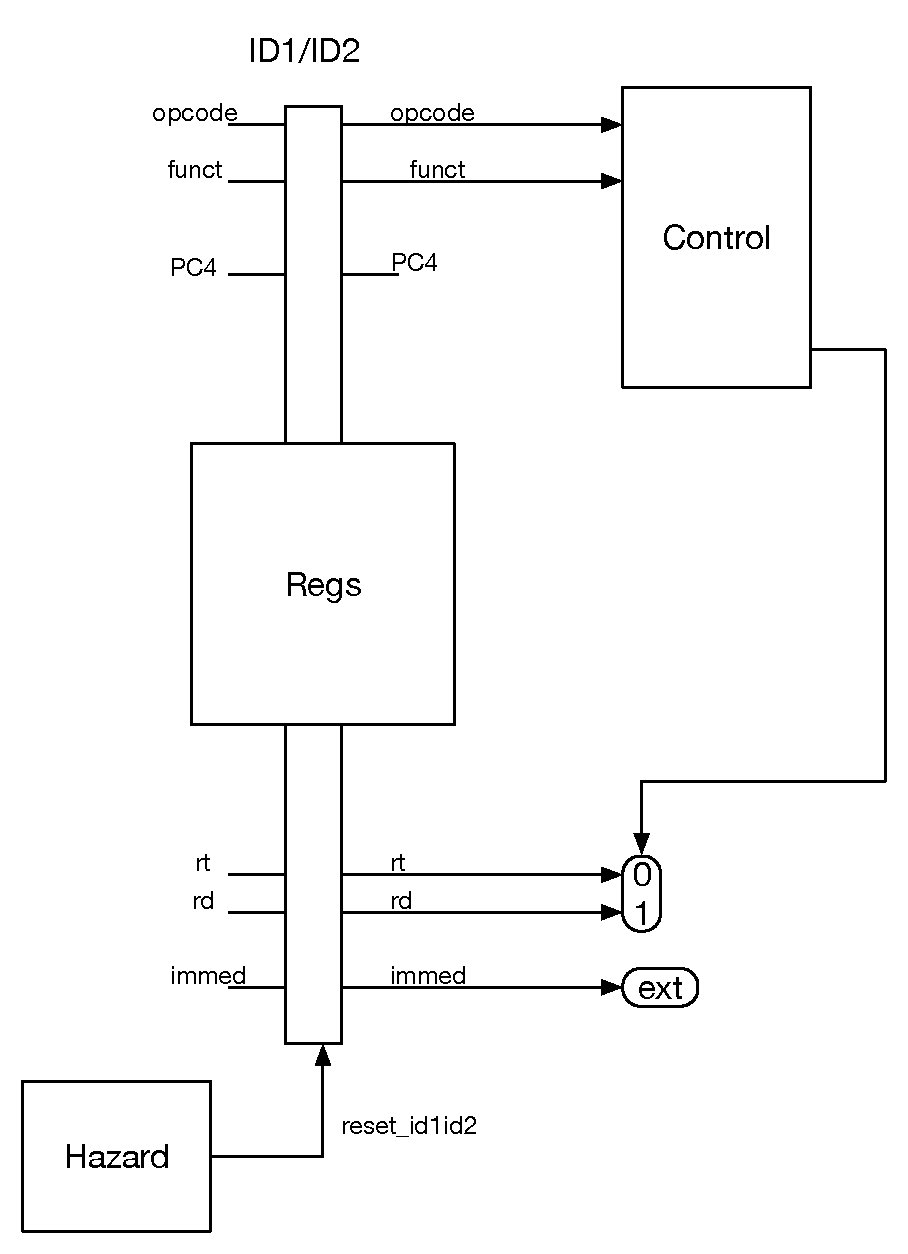
\includegraphics[width=100mm,scale=1]{ID1ID2ex1.pdf}
 \caption{\\ Registo ID1/ID2}
 \label{fig:eer}
\end{figure}

O inicio da leitura de registos tem inicio em ID1 e termina em ID2 (como podemos verificar na figura 1), sendo a fase ID1 apenas utilizada para esse efeito, sendo que tudo o que se resolvia em ID se resolve em ID2, como por exemplo a unidade de Controlo, o extend e o Mux.

Para este primeiro exercício criou-se um registo novo ID1/ID2, que toma como entradas o \textit{opcode}, o \textit{funct}, o \textit{immed}, o \textit{rt} e o \textit{rd} vindos do decoder de ID1, sendo portanto as saídas estas mesmas portas. Existe também uma entrada vinda da unidade de Hazard, \textit{reset\_id1id2}, para fazer reset a este registo aquando da necessidade de existirem stalls ou branchs.

Na unidade de hazard foram feitas algumas alterações para que estes fossem resolvidos em ID2, que anteriormente eram resolvidos em ID. A única diferença é que são os registos em ID2, rs e rt, que definem a existência de hazard tendo em conta as fases mais avançadas da pipeline, como EXE, MEM e WB.

\newpage
\section{Exercício 2}

Neste segundo exercício, foi-nos proposto para que todos os saltos condicionais e incondicionais, fossem resolvidos em ID2. Para isso foi criada uma unidade de branch, que através de entradas como \textit{opcode}, \textit{rsdata}, \textit{rtdata}, \textit{branch}, \textit{target}, \textit{imm\_ext} e \textit{PC4}, calcula o \textit{branchTaken}, que nos diz se existe salto ou não, e o \textit{branchTarget} (Figura 2).

\begin{figure}[!htb]
\center
 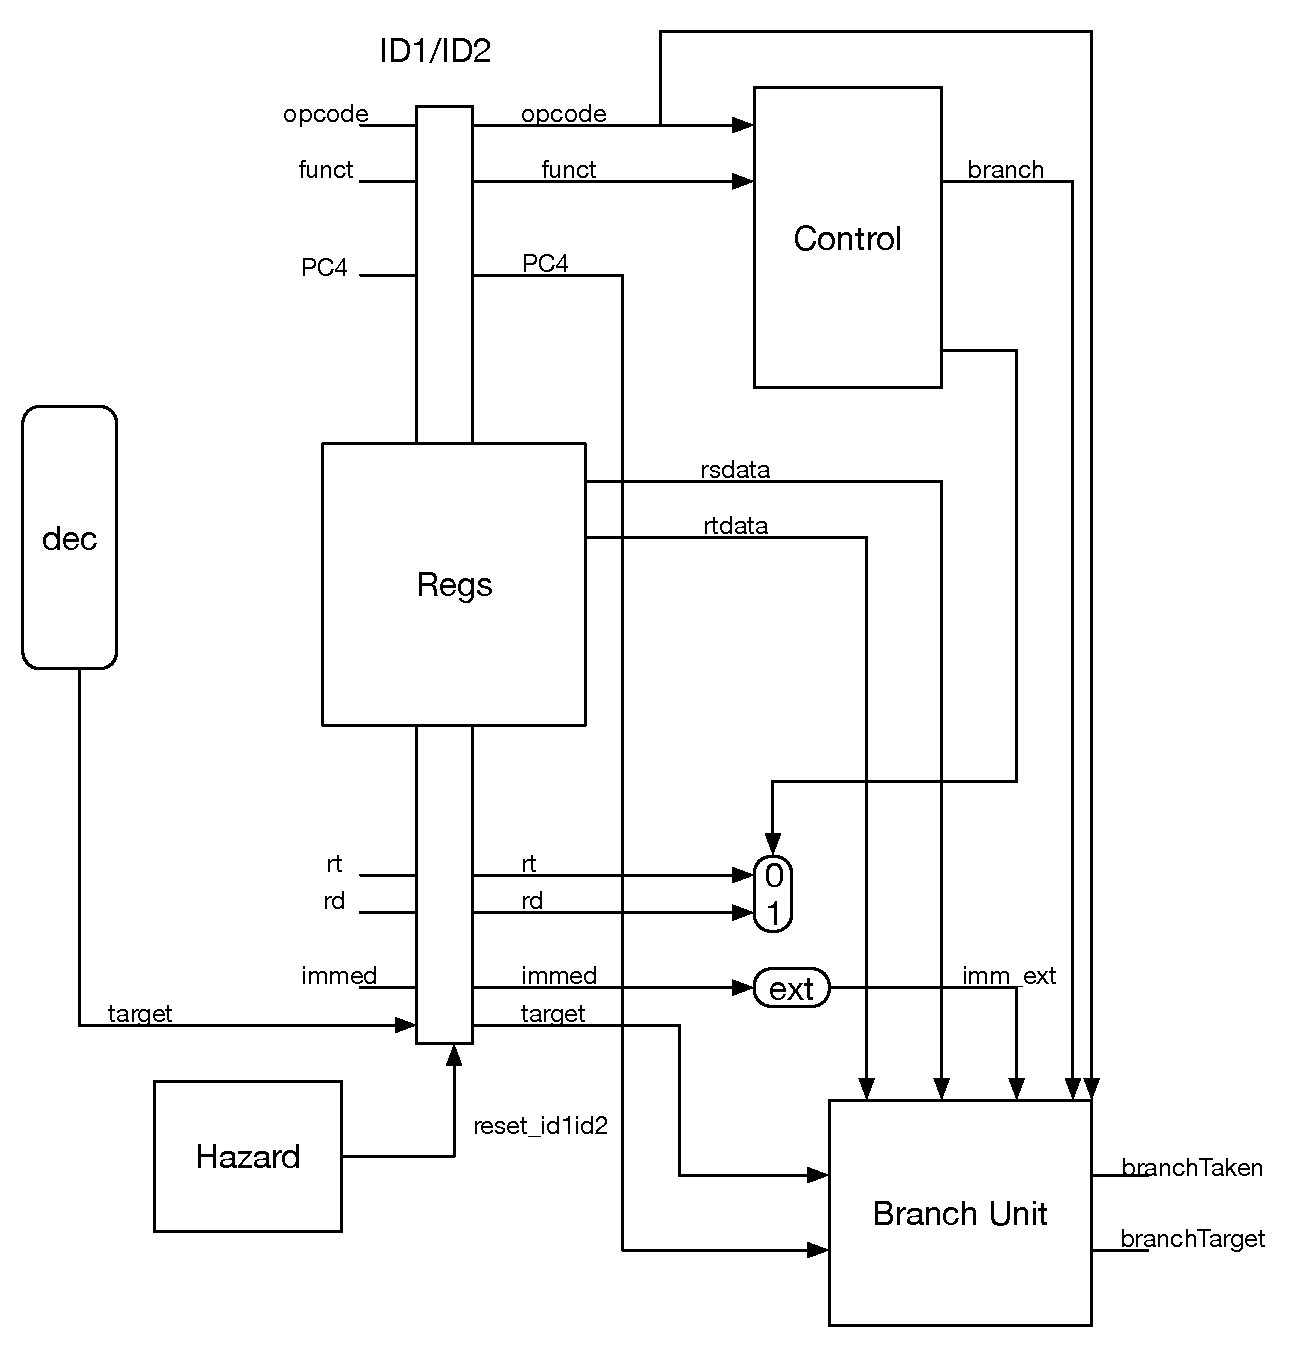
\includegraphics[width=100mm,scale=1]{ID1ID2ex2.pdf}
 \caption{\\Registo ID1ID2 com Branch Unit}\label{fig:eer}
\end{figure}

\subsection{Unidade de Branch}

Para que os saltos fossem resolvidos em ID2, foi necessário na unidade de branch resolver os mesmos. Para isto dentro da unidade de controlo, alterou-se a informação que a saída de branch possuí. Disponibilizaram-se mais bits para que esta saída indique na unidade de branch o tipo de salto que estamos a resolver.

Posto isto na unidade de branch, efectuam-se 6 casos diferentes:

\begin{itemize}
\item BEQ: compara se o valor de \textit{rsdata} é igual ao de \textit{rtdata}
\item BNE: compara se o valor de \textit{rsdata} é diferente de \textit{rtdata} 
\item BGTZ: compara se o valor de \textit{rsdata} é maior que zero
\item BLEZ: compara se o valor de \textit{rsdata} é menor ou igual a zero
\item JUMP: salta para o target da instrução
\item JR: salta para o valor de \textit{rsdata}
\end{itemize} 

Sendo os saltos resolvidos em ID2, foram removidos de fases mais avançadas unidades que não seriam mais utilizadas, como por exemplo o \textit{sl2} e a unidade de adição para branch em EXE e o \textit{and} em MEM. Os portos \textit{PC4} e \textit{branch} também deixaram de ser propagados para as fases seguintes à ID2.

\subsection{Unidade de Hazard adaptada para a nova resolução de saltos}

Para que instruções que entrem de forma errada na pipeline quando um branch ocorre sejam descartadas excepto a seguinte (delayed branch slot), foi necessário alterar na unidade de Hazard as fases às quais é necessário fazer reset. Desta feita quando a nossa unidade de Hazard trata de descartar instruções que entrem de forma errada na pipeline e de colocar stalls aquando da ocorrência destes.

\section{Tecnologias usadas}

As tecnologias usadas no desenvolvimento do IEDCS Server, foram: Django + Python e AngularJS + JS. O Django dá a possibilidade de usar proteção contra \href{https://docs.djangoproject.com/en/1.8/ref/csrf/}{CSRF} usando um token e um middleware que obriga que o cliente envie este token sempre que faz um pedido para a aplicação.  

O Angular.JS já tem suporte para enviar o CSRF token, sempre que recebe um \textit{Set-Cookie CSRFToken = XXX} na resposta do servidor, irá gravar esse csrf token num cookie no browser do utilizador e irá enviar sempre que for feito um pedido.

Já o nosso Player foi feito usando Java e JavaFX. No java tivemos de usar uma biblioteca para fazer os pedidos HTTP e HTTPS exterior, neste caso usámos a org.apache.http. Esta biblioteca não tem suporte para uso de um CSRF de forma correta, por isso, tivemos de implementar uma classe (Requests.java) que gerisse uma ligação HTTP e guardasse o seu estado de sessão. Nesta classe enviamos um X-CSRFToken no Header do pedido.

No servidor, também temos a proteção contra SQL Injection e XSS ataques pois fazemos uso dos métodos disponibilizados pelo Django para manipulação de modelos da base de dados. Já o AngularJS não permite que seja injetado código JS nem HTML sem intenção do programador da aplicação.

Como usamos Python e Java já temos proteção contra buffer overflows e mesmo assim tivemos cuidado para não fazer implementações que comprometessem o estado tanto do servidor como do player, como por exemplo, uma saída inesperada devido a um erro.

\section{Casos de utilização}

\subsection{Registo de um utilizador}

Um registo de um utilizador é feito na página web disponibilizada pelo IEDCS. Ao gravar na base de dados a password é gravada com um segundo PBKDF2 e SHA256, o que torna computacionalmente trabalhoso obter as passwords dos nossos utilizadores caso a base de dados seja exposta. Ao fazer login, tanto no Player como na interface Web é aplicado PBKDF2 com HMAC e SHA1 para caso o HTTPS seja comprometido, as passwords não sejam enviadas em claro pela rede ou  caso se esteja a usar HTTP.

\begin{center}
	\textbf{Password = PBKDF2(Password, Password, 500)}
\end{center}

Não existe nenhuma criação da chamada UserKey, esta no entanto, é gerada para cada livro por cada utilizador quando ele solicita pela primeira vez a leitura do mesmo. Optou-se por fazer um UserKey por Livro para dificultar ainda mais a tarefa a quem tente comprometer o nosso sistema de IEDCS.

\begin{figure}[!htb]
\center
 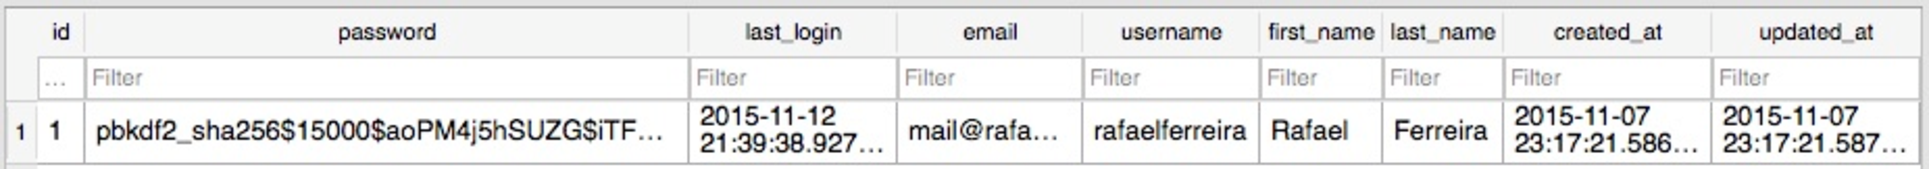
\includegraphics[width=150mm,scale=1]{pbkdf2_saved.pdf}
 \caption{\\Password guardada com PBKDF2 e SHA256}
 \label{fig:eer}
\end{figure}

\subsection{Registo de um device}
Quando um player é utilizado pela primeira vez num determinado device, no momento do login de um utilizador, o Device é registado na base de dados com os seguintes parâmetros:

\begin{itemize}
\item Identificador único
\item Modelo de CPU
\item Modelo do PC
\item IP
\item País
\item Hora
\item Host name
\item Chave pública do Device
\end{itemize}

	No Player é usado a biblioteca sigar para obter os dados do device. O País é obtido no servidor através do IP recebido pelo mesmo.
	A cada utilizador também são associados os vários devices por onde já se conectou ao servidor.
	Caso no momento do login, o device já exista na base de dados, este é atualizado com os novos dados recebidos, tal como a hora, IP, entre outros já especificados.

\subsection{Aquisição de um livro}

No momento de aquisição do livro não há nenhuma cifra, apenas um registo na base de dados que o utilizador adquiriu um livro.

\subsection{Restrições na visualização de um livro}

Para a visualização de um livro criaram-se dois tipos de restrições, por país e por hora de utilização.

Isto permite que os conteúdos não possam ser acedidos a qualquer momento e em qualquer lado caso existam restrições nesse livro.

\begin{figure}[!htb]
\center
 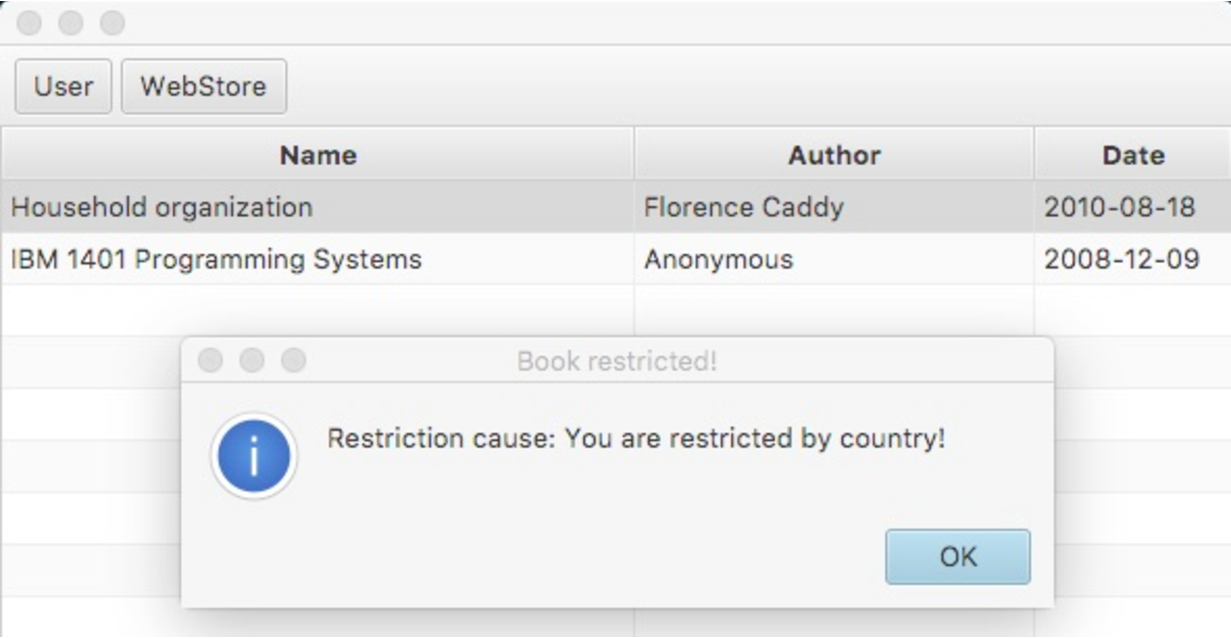
\includegraphics[width=100mm,scale=1]{country_restriction.pdf}
 \caption{\\Restrição apresentada tendo em conta o país do utilizador}
 \label{fig:eer}
\end{figure}

\subsubsection{Gestão de restrições}

Para ser mais simples gerir as restrições por parte do administrador do sistema foi criado uma interface de linha de comandos com várias possibilidades. 
Para adicionar uma restrição a um livro:
\shellcmd{python manage.py restriction add restrict{\_}book book{\_}identifier\linebreak restriction{\_}name}
Para adicionar uma nova restrição no sistema:
\shellcmd{python manage.py restriction add restriction restriction{\_}name\linebreak restrictionFunction cause}
Para remover uma restrição a um livro:
\shellcmd{python manage.py restriction rm restrict{\_}book book{\_}identifier\linebreak restriction{\_}name}
Para listar os livros disponíveis:
\shellcmd{python manage.py restriction list books}

\section{Instalação}

Para uso e instalação do nosso sistema, criou-se uma pasta /installation que tem um ficheiro \textit{Vagrantfile} que permite criar um servidor ubuntu trusty 64bits que cria uma pasta partilhada neste em /var/www que irá servir para lançar o servidor IEDCS com recurso ao Apache2. O ficheiro \textit{server-bootstrap.sh} servirá para instalar todas as bibliotecas necessárias, todos os pacotes do python, a configuração do Apache2 para o nosso site que está no ficheiro \textit{iedcs.rafaelferreira.pt.conf} e \textit{default-ssl.conf}, também para instalar os certificados necessários para o HTTPS nas pastas usadas para esse efeito e para criar a base de dados com os livros e restrições exemplo.
	
O ficheiro \textit{iedcs.rafaelferreira.pt.conf} serve apenas para redirecionar todos os pedidos HTTP para HTTPS. O ficheiro \textit{default-ssl.conf} tem todas as configurações necessárias para o uso de HTTPS e para usar o modWSGI do Apache2 para o Django.

Criou-se um package de settings para o Django para ter definições de development e outras de servidor. Usando o hostname do servidor sabemos em que modo deve estar, sendo assim nesse servidor iniciado com Vagrant o servidor estará em modo produção, ou seja, não irá lançar output de debug para o utilizador.

O \textit{install{\_}cert.sh} é usado para criar uma keystore que será usada pelo Java para armazenar os certificados em que ele confia ao usar HTTPS.	
	
Para usar o servidor, além de ter o \href{https://www.vagrantup.com/downloads.html}{Vagrant} intalado, é apenas necessário fazer:
\shellcmd{vagrant up}

A password caso seja pedida é sempre vagrant e para aceder à máquina é apenas necessário fazer: \shellcmd{vagrant ssh}

O site pode ser acessível em: \url{https://iedcs.rafaelferreira.pt/}

Para fazer download do Player apenas é preciso registar na webstore e depois clicar em "Player" que será feito o download do Player. A implementação do Player está apenas disponível para Mac OS X, com uma aplicaçãnative application  tendo como base uma aplicação JavaFX. Testado com o java version "1.8.0{\_}60".

\section{HTTPS}
Para criar um certificado criou-se uma chave privada RSA com:

\textit{openssl req -new -newkey rsa:2048 -nodes -keyout server.key -out server.csr}

\textbf{output:} /installation/ssl/generating.txt

O certificado foi depois emitido usando a \href{https://www.instantssl.com/free-ssl-certificate.html}{Free SSL}.

Como foi criado um domínio que aponta para o endereço \textit{192.168.33.10} que é o endereço local do servidor IEDCS inicializado pelo Vagrant.

\section{Problemas identificados na primeira entrega}

Nesta primeira entrega, identificaram-se alguns problemas, nomeadamente no corrompimento do HTTPS, através da troca da keystore onde são guardados os certificados confiáveis, podendo assim injetar todos os certificados que se deseja de forma a que seja possível intercetar as comunicações entre o servidor e o Player. Para isso sabemos que o utilizador pode descompilar o código do Player, analisar o nosso processo de cifra e o código. Com isto ele poderá descobrir que usamos um ficheiro cacerts.keystore para o Java confiar apenas no nosso certificado, pode então modificar essa keystore e o cliente ao fazer download pode ser-lhe dada uma versão corrompida, mas sem estar corrompida no código, apenas no cacerts.keystore. Se estiver presente outro certificado que o atacante domine, ele pode intercetar as comunicações HTTPS e aceder às comunicações que estão a ser trocadas entre a vítima que está a usar o Player e o nosso Servidor e assim, pode, obter o Random2 e derivar o n (este é enviado inicialmente num Header), o book identifier e o rd2 que é enviado pelo servidor no pedido de challenge ao cliente. O texto “ua” é possível de ser obtido descompilando o código. Após isto, ele pode cifrar com AES e obter a file key. Com isto, consegue decifrar o nosso livro cifrado.

Outra possibilidade seria um atacante/cliente que usasse ferramentas de análise de memória para obter o livro cifrado, e todas as outras variáveis que estão expostas em Runtime.

\subsection{Soluções}

\begin{itemize}
\item Assinar o Player com uma chave assimétrica assim como o ficheiro cacerts.keystore.
\item Autenticando ambas as entidades no momento em que é negociada o HTTPS entre o cliente e o servidor (2º parte do trabalho).
\item Sessão para a file key usada ser sempre diferente tendo em conta a sessão, proibindo a reutilização da file key em vários devices e players.
\item Cifra por página, ou seja, a paginação ser realizada no lado do servidor.
\end{itemize}

\end{document}

\newpage
\section{Conclusão}

Esta conclusão não é uma conclusão final, pois este projeto será realizado em duas partes.
Sendo assim vamos optar por nesta conclusão dizer principalmente as implementações futuras e problemas encontrados.

O principal problema encontrado, foi fazer a decifra no lado do Java, depois de a cifra estar feita do lado do Python, pois muitas tecnologias disponibilizadas por este não estão disponíveis diretamente no Java, o que nos obriga a utilizar bibliotecas externas o que nem sempre é bom, pois podemos estar a acrescentar problemas ao sistema. 

As implementações futuras que não conseguimos implementar a tempo nesta fase do projeto, mas que contudo poderão fazer parte da próxima são:
\begin{itemize}
\item Uma sessão única sempre o device atualiza os seus dados. Este atualiza os seus dados sempre que o utilizador efetua um inicio de sessão, tenta ler um livro e muda de página. Esta solução faria com que a cifra do conteúdo do livro apenas fosse válida durante a sessão, pois assim que fosse efetuado um outro challenge com o servidor a sessão iria mudar e o Player não iria conseguir fazer a decifra.
\item A solução apresentada acima, obriga a que seja feita a cifra página a página, consoante a sessão do Player, Device e utilizador.
\item Outra ideia que nos surgiu, foi apresentar ao utilizador as duas páginas iniciais de cada EBook (Sample) de forma gratuita.
\end{itemize}

